\section{Why Visible Events Can Have Ambiguous Sources}
\label{sec:narrative-information}

The continuous results raise a separate physical question: can these
measurements distinguish the candidate sources at all? A good state
estimate does not answer it. Different interventions can produce similar
histories after fitting their severity and initial state
\cite{eriksson2013diagnosability,scharf1994matched}.

For a response $s_h$ at a specified severity and context, its distance to
an admitted competitor is
\begin{equation}
 d_h^2=\min_{j\ne h}\ \min_{\eta_j\in\mathcal A_j}
      \|s_h-s_j(\eta_j)\|_{\Sigma^{-1}}^2.
 \label{eq:narrative-separation}
\end{equation}
The set $\mathcal A_j$ specifies allowed severity, sign and nuisance
coordinates. If zero severity is admitted, different support families can
meet at the no-event boundary. Unrestricted amplitude minimization would
then give a misleading source-separation interpretation. Under a common
Gaussian law, coincident means cannot be distinguished at that
intersection. Small distances indicate a noise-sensitive problem, not a
universal error formula or an online uncertainty certificate.

A separate completed load-only experiment illustrates this limit. It uses
32 rectangular voltage/current coordinates, known onset and known operating
context. Its original amplitude-marginalized batch likelihood compares 137
zero-, one- and two-source supports on \GlobalPhysicalTrajectories{} fresh
nonlinear trajectories. It is a different estimator and evidence contract
from the causal bank.

\begin{figure*}[t]\centering
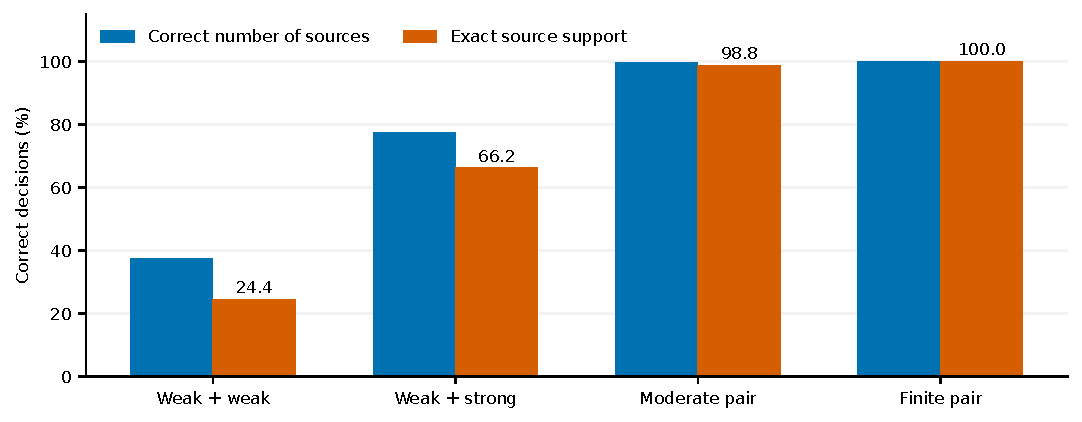
\includegraphics[width=.93\textwidth]{figures/generated/narrative_resolution.pdf}
\caption{Auxiliary source-resolution evidence, separate from the continuous estimator. In the known-onset load study, cardinality identifies the number of sources and exact support identifies their locations. Both improve with severity, but weak pairs remain difficult. These are results of the original 137-support batch likelihood, not unknown-onset R11 accuracy or a test of other event families.}
\label{fig:narrative-resolution}\end{figure*}

Exact-support Top-1 increases from \GlobalWeakTopOne{} for weak pairs to
\GlobalFiniteTopOne{} for finite pairs (Fig.~\ref{fig:narrative-resolution}).
A visible intervention therefore need not yield a reliable location.
Longer history can help separate trajectories, without guaranteeing unique
attribution for every source, severity or sensor placement. This analysis
interprets ambiguity; it is not a calibrated abstention rule in R11.
Detailed state-reconstruction studies remain supporting evidence rather
than extra event-diagnosis scores.
